% !TEX root = main.tex

\section{System}
\label{sec:system}
%In diesem Kapitel werden die wesentlichen Komponenten der Implementierung erläutert.
%
%Die Aufnahme der Medienquellen wird durch die getUserMedia-API über das \textit{MediaStream}-Objekt ermöglicht.
%ToDo

\subsection{WebSockets}
\label{subsec:websockets}
Für das Signaling ist eine Kommunikation über mehrere Schritte hinweg notwendig.
Damit diese ohne eine Vielzahl an HTTP-Anfragen und komplexer serverseitiger Vorkonfiguration realisiert werden können, wird client- und serverseitig
die WebSocket-API\parencite{WebSocketSpec} genutzt\footnote{Serverseitig wird die WebSocket API von Java genutzt\parencite{JavaEEWebSocket}}.
Da WebRTC allerdings keinen Transport-Mechanismus für die Signaling-Informationen spezifiert, ist es auch möglich die Informationen über
XMLHttpRequests zu versenden (sog. Ajax-Requests).
WebSockets ermöglichen die bidirektionale Client-Server Kommunikation.
Dabei kann der Client dem Server Nachrichten senden und ereignisorientierte Antworten erhalten,
ohne Antworten durch HTTP-Anfragen abzufragen\parencite{WebSocketMDN}.
Die Nachrichten werden dabei im JSON-Format ausgetauscht.
Folgende Ereignisse können, sowohl client- als auch serverseitig, ausgelöst werden:
\begin{itemize}
    \item OnOpen()
    \item OnMessage()
    \item OnClose()
    \item OnError()
\end{itemize}

\subsection{SDP (Session Description Protocol)}
\label{subsec:sdp}
SDP ist ein Standardformat um eine \textit{peer-to-peer} Verbindung zu beschreiben und wird u.A. von WebRTC genutzt um Sitzungen von \textit{peers} zu beschreiben.
Es enthält Informationen zur verwendeten Codec, den IP-Adressen der \textit{peers}, und zu Zeitabschnitten von Video- und Audiodaten\parencite{MDNSdp}.
\begin{figure}[!ht]
%figure full paperwidth and trim the left and right empty space from it
    \makebox[\textwidth]{
        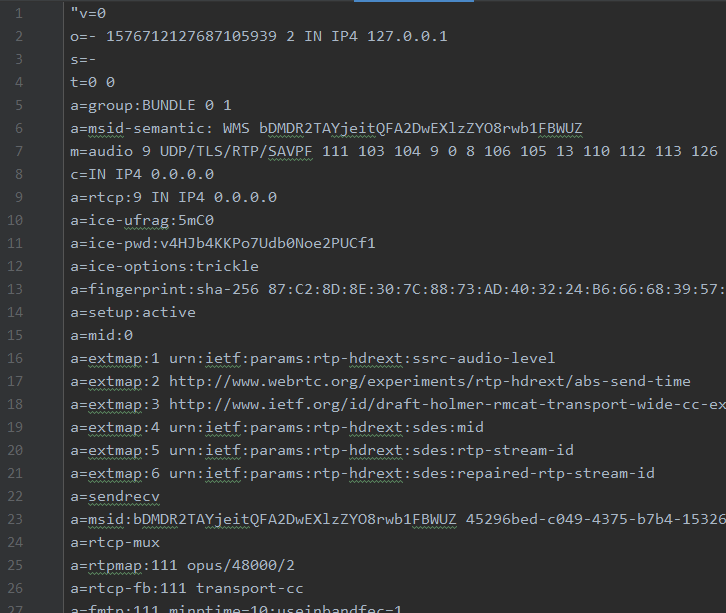
\includegraphics[trim = 16mm 0mm 16mm 0mm,width=0.7\paperwidth]{resources/sdp-localhost-example.png}
    }
    \caption{Ausschnitt einer SDP-Nachricht zwischen zwei \textit{peers} auf \textit{localhost}}
    \label{fig:sdp-localhost}
\end{figure}

\subsection{ICE (Interactive Connectivity Establishment)}
\label{subsec:ice}
ICE ist ein von WebRTC genutztes Framework um zwei Peers miteinander zu verbinden, unabhängig von der vorhandenen Netzwerk-Topologie. \parencite{RFCIce}
Das ICE-Protokoll ermöglicht das finden und etablieren einer Verbindung zwischen zwei \textit{peers}, selbst wenn beide eine Netzwerkadressübersetzung(NAT)
nutzen, um eine öffentliche IP Adresse mit anderen Geräten in ihrem Netzwerk zu teilen.
Dafür kann im Konstruktor eines RTCPeerConnection-Objektes ein STUN und/-oder TURN Server angegeben werden.

Der Algorithmus des Frameworks versucht dabei immer den Pfad mit der niedrigsten Latenz zu nutzen um die beiden \textit{peers} zu verbinden.
Dabei probiert er die folgenden Optionen in der genannten Reihenfolge:

\begin{enumerate}
    \item Direkte UDP Verbindung (in diesem Fall wird ein STUN Server genutzt um die IP-Adresse des \textit{peers} innerhalb des Netzwerkes zu finden)
    \item Direkte TCP Verbindung, über den HTTP-Port
    \item Direkte TCP Verbindung, über den HTTPS-Port
    \item Indirekte Verbindung über einen TURN Server (wenn eine direkte Verbindung fehlschlägt, bspw. wenn ein \textit{peer} hinter einer
    Firewall liegt, die die NAT-Traversierung blockiert)\parencite{MDNIce}
\end{enumerate}

\subsection{STUN und TURN Server}
\label{subsec:natturnserver}
STUN (Session Traversal Utilities for NAT) ist ein Hilfsprotokoll um Daten durch ein NAT (Network Address Translator) an das Ziel zu übermitteln.
Es gibt die IP-Adresse, den Port, und den Verbindungsstatus des Computers hinter dem NAT zurück\parencite{MDNStun} und ermöglicht somit
eine direkte Kommunikation der beiden \textit{peers}.
\newline
TURN (Traversal Using Relays around NAT) ist ein Protokoll das einem Computer - hinter einem NAT oder einer Firewall - ermöglicht Daten zu senden und empfangen.
Dabei wird der gesamte Traffic der beiden \textit{peers} während den \textit{gesamten} Kommunikationszeitraums über den TURN-Server an den jeweils anderen \textit{peer} weitergeleitet.
Der TURN-Server muss dabei in der Regel öffentlich zugänglich sein.
TURN-Server werden dann genutzt, wenn eine direkte Kommunikation der \textit{peers} durch eine sehr restriktive Firewall nicht möglich ist\footnote{
    Bei permanent hohem Traffic der \textit{peers} kann die Nutzung eines externen TURN-Servers ein Performance-Bottleneck darstellen.}\parencite{MDNTurn}.

\subsection{Signaling}
\label{subsec:signaling}

Ein Signaling-Server fungiert als Mittelsmann und ermöglicht es zwei \textit{peers} sich zu finden und eine Verbindung aufzubauen, indem
er die Signaling-Daten jeweils an den entsprechenden {peer} weiterleitet.
Dabei muss der Server den Inhalt der Signaling-Nachrichten nicht verstehen
\footnote{Der Inhalt der Signaling-Nachrichten kann daher als Black-Box gesehen werden.} können, solange
der jeweilige \textit{peer} die Nachricht erhält und an sein ICE-System (siehe Abschnitt \textit{ICE}) weitergibt.
WebRTC nutzt für die Inhalte der Signaling-Nachrichten das \textit{Session Description Protocol (SDP)} und
für die Kommunikation mit dem Signaling-Server werden \textit{WebSockets} empfohlen.

Zu Beginn des Signaling Prozesses initialisiert Peer A ein RTCPeerConnection-Objekt und erstellt ein Offer mithilfe der CreateOffer()-Methode.
Das Offer enthält seine Session-Description im SDP-Format und wird über den Signaling-Server an Peer B geschickt, welcher auch ein RTCPeerConnection erstellt.
Dieser verarbeitet das Offer und dessen Inhalt und reagiert mit einer Answer, die wiederrum die Session Description von Peer B enthält.

Nachdem Peer A die Answer verarbeitet hat, haben beide \textit{peers} das jeweilige RTCPeerConnection-Objekt mit ihrer und der Session-Description des anderen
Peers gefüllt, sowie den Audio-und Videodaten der jeweiligen Medienquelle als MediaStream-Objekt.

Beide \textit{peers} kennen nun die IP-Adresse des jeweils anderen und die zu nutzenden Codecs, wissen noch allerdings nicht wie die
Mediendaten übertragen werden sollen.
Um dies zu ermitteln, wird das ICE-Framework von WebRTC genutzt.

\begin{figure}[!ht]
%figure full paperwidth and trim the left and right empty space from it
    \makebox[\textwidth]{
        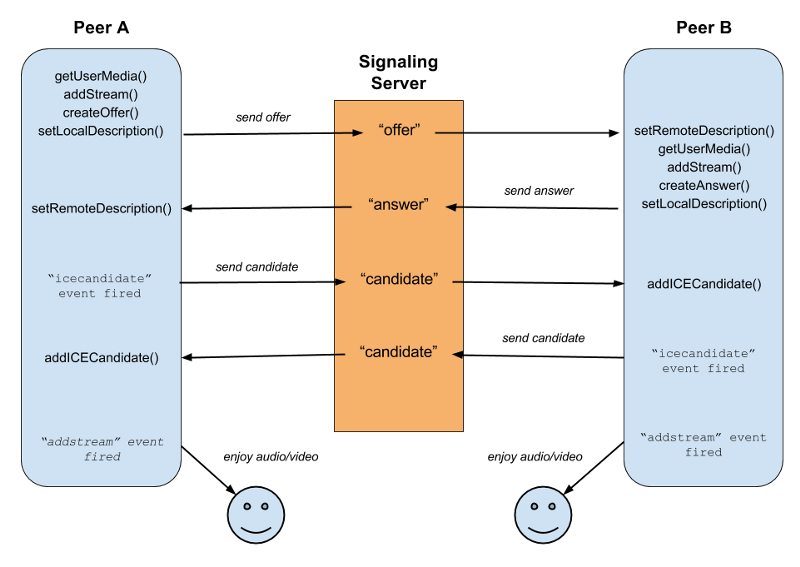
\includegraphics[trim = 16mm 0mm 16mm 0mm,width=0.8\paperwidth]{resources/WebRTC-Signaling.png}
    }
    \caption{WebRTC Signaling Ablauf, \parencite{SatanasGithub}}
    \label{fig:webrtc_signaling}
\end{figure}

Die \textit{peers} tauschen ICE-Kandidaten aus um die aktuelle Verbindung zu verhandeln.

Jeder ICE-Kandidat beschreibt eine Methode die der sendende \textit{peer} zur Kommunikation nutzen kann.

Beide \textit{peers} senden Kandidaten in der Reihenfolge, in der sie entdeckt werden, und senden solange bis sie keine Vorschläge
mehr haben - selbst wenn die Mediendaten bereits übertragen werden.
Jede ICE-Nachricht schlägt ein Kommunikationsprotokoll (TCP oder UDP), IP-Adresse, Port und andere Informationen vor, die benötigt werden
um eine Verbindung aufzubauen.
Dies beinhaltet auch NAT .

Sobald sie sich auf einen beidseitig-kompatiblen Kandidaten geeinigt haben, wird das SDP des Kandidaten von jedem Peer genutzt um eine
Verbindung aufzubauen, durch welche die Mediendaten ausgetauscht werden.

Falls Sie sich später auf einen besseren Kandidaten (normalerweise mit besserer Performance) einigen, ändert sich das Format des Datenstroms.

\parencite{MDNSignaling}

